% =========================================================
% Section 4 — Evaluation Framework (claims aligned)
% =========================================================
\begin{figure*}[t]
  \centering
  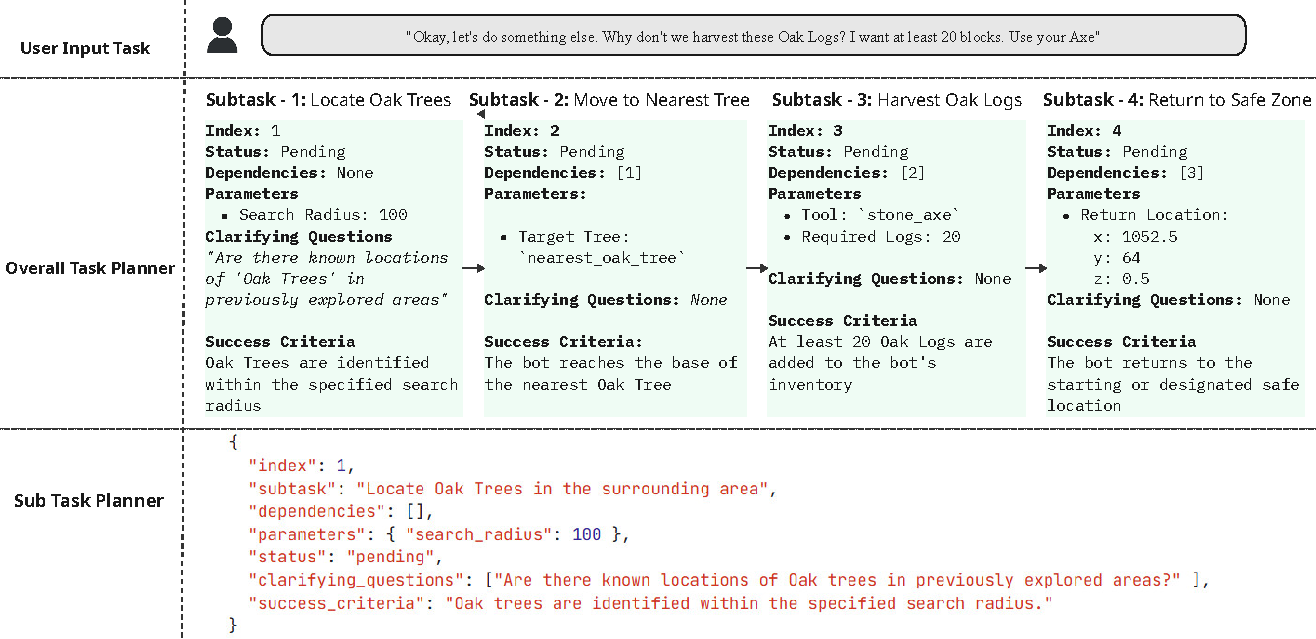
\includegraphics[width=\textwidth]{Sections/Figures/user_input_fig.pdf}
  \caption{Planning surfaces for “harvest oak logs.”
  \panel{a} Chat request routed to \texttt{task(request)}.
  \panel{b} Short, legible plan with dependencies.
  \panel{c} Subtask record with defaults (e.g., \texttt{search\_radius}=100) and its clarifying question.}
  \label{fig:planner}
\end{figure*}

\section{Evaluation Framework}
\label{sec:framework}

We now describe the evaluation framework that turns the constraints and task templates into a reproducible harness for testing LLM agents in \emph{Minecraft} via Mineflayer. Figure~\ref{fig:atpes-hero} summarizes the pipeline. The framework is model-agnostic: an LLM proposes a short plan, asks at most one targeted clarifying question when a required parameter is unbound, generates Mineflayer-compatible code to act, and is judged from bounded, in-world evidence. In this paper we instantiate the framework with GPT-4o; Section~\ref{sec:evaluation} reports that snapshot.

\SubsectionFigure{Sections/Figures/user_intent.pdf}
{Routing and planning. Ingress via chat or control buttons is parsed into intents (\emph{update memory}, \emph{conversation}, \emph{task}, \emph{control}). Tasks flow to a planner that decomposes requests and binds missing slots with a single, contextual question when needed.}
{fig:user-intent}

\noindent
\textbf{Observation and action contract.}
Perception and control are constrained to public, in-game interfaces exposed by Mineflayer. The agent can read recent chat, its inventory and equipment, and nearby entities and blocks within currently loaded chunks (a practical proxy for line-of-sight). It can navigate, mine, craft, place, interact, transfer items, and return/drop off; destructive operations require an explicit confirmation step. A bounded-knowledge policy forbids admin commands (e.g., \texttt{/give}, \texttt{/teleport}), global map/seed introspection, and bulk scans beyond loaded chunks; attempts that trigger a forbidden call are marked invalid. See Fig.~\ref{fig:user-intent} for the routing pathway that feeds planning.

\begin{center}
  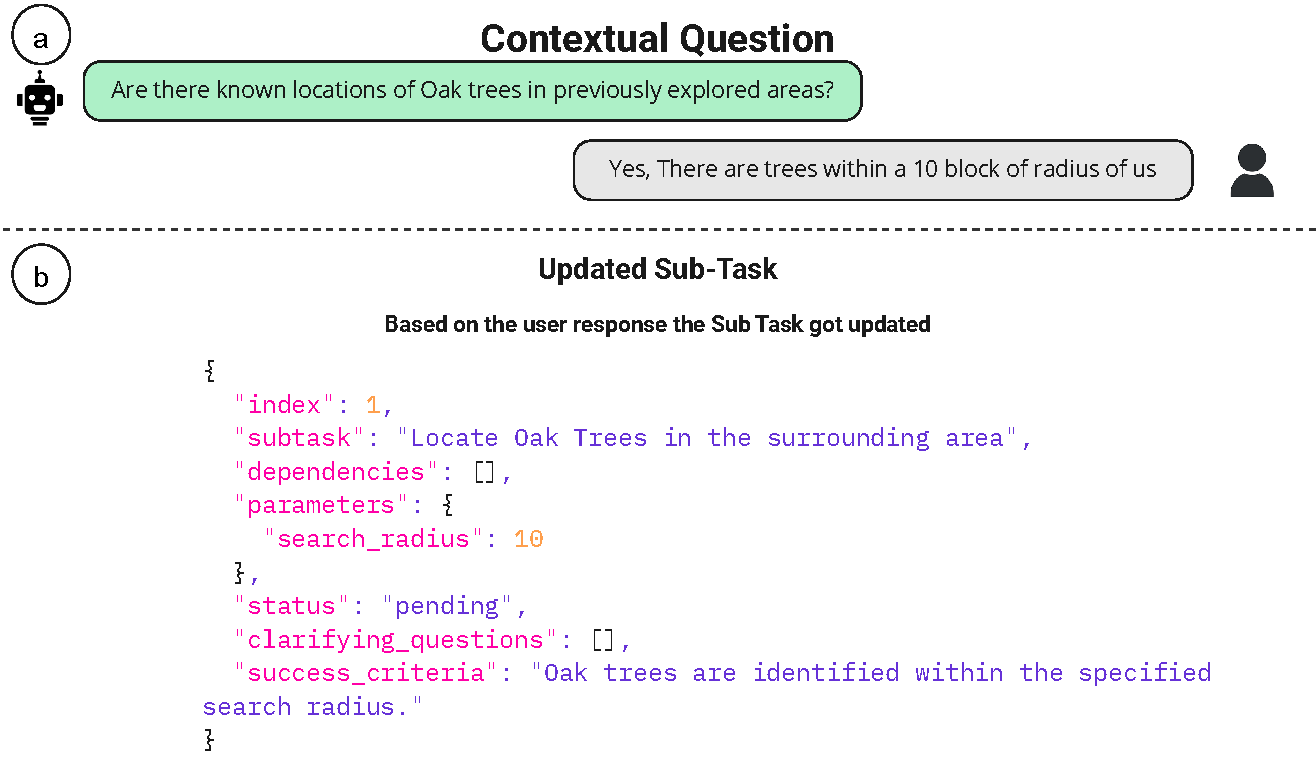
\includegraphics[width=\columnwidth]{Sections/Figures/contextual_qn.pdf}
  \captionof{figure}{Mixed-initiative example. \panel{a} The planner asks whether oak trees are within a known radius; the player replies “within 10 blocks.” \panel{b} The plan updates \texttt{search\_radius} from 100 to 10 and stores the preference with provenance \textit{told}.}
  \label{fig:context-qn}
\end{center}

\noindent
\textbf{Plan preview and clarification.}
Player requests arrive through chat and are routed to \texttt{task(request)} when they imply action. Before any execution, the framework renders a one-line plan preview and exposes precondition checks (Fig.~\ref{fig:planner}). If a required slot (e.g., tool variant, drop-off location, or search radius) is not bound by context, the agent asks \emph{one} targeted question rather than guessing; the answer is applied immediately to the active plan and written to memory with provenance for later reuse (Fig.~\ref{fig:context-qn}).

% Judging figure appears earlier in pagination (Figure 6), but we will
% reference Code Review (Figure 7) first in the text to keep the logic flow.
\noindent
\textbf{From template to plan.}
Given a user goal and the corresponding task template (Appendix~\ref{app:tasksuite}), the framework compiles a short plan with three to five subtasks (Fig.~\ref{fig:planner}\panel{b}). Each subtask is represented by a compact record (Fig.~\ref{fig:planner}\panel{c}) specifying its name, dependencies, required parameters, a clarifying question issued only when a required parameter is missing, and a success criterion. These structures are logged to make plan deltas auditable (e.g., \texttt{search\_radius}: 100$\rightarrow$10).

\noindent
\textbf{Execution with review.}
Plans execute through generated JavaScript against Mineflayer. A lightweight reviewer checks basic API usage and guard conditions; retries are capped ($K{=}2$–$3$) to prevent runaway loops. Approved code is dispatched, and the runtime emits compact progress toasts so players can track what is happening without breaking flow (Fig.~\ref{fig:code-review}).

\begin{center}
  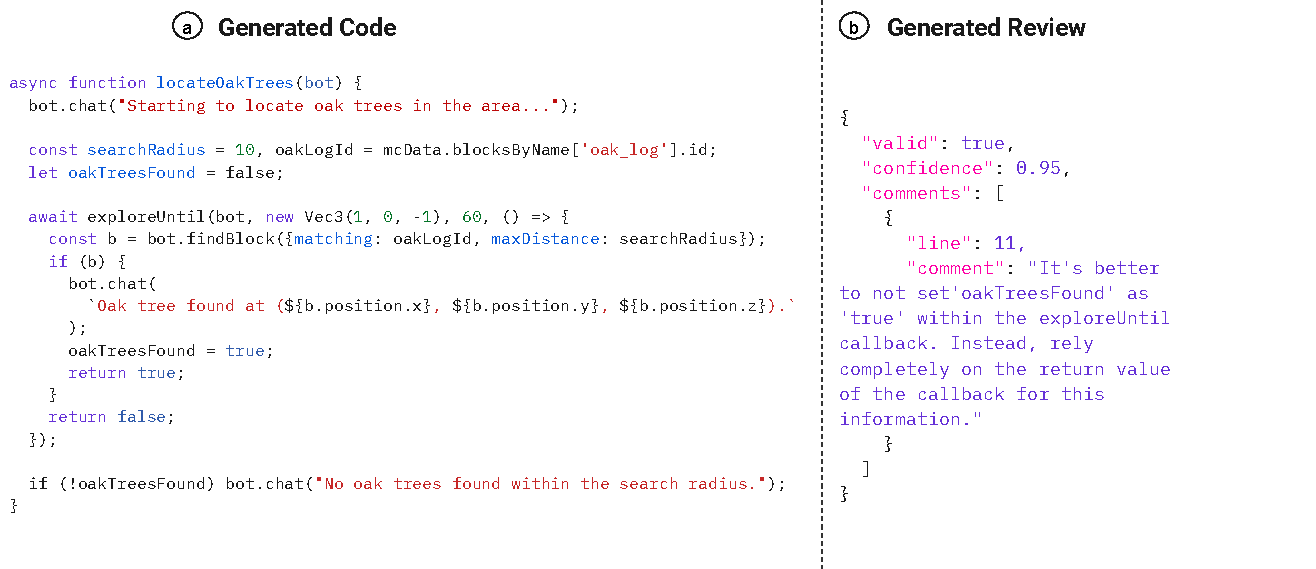
\includegraphics[width=1.1\columnwidth]{Sections/Figures/code_and_review.pdf}
  \captionof{figure}{Code generation and review. \panel{a} Generated JavaScript reflects updated parameters (e.g., \texttt{searchRadius = 10}) and emits legible chat updates. \panel{b} Reviewer feedback flags robustness issues before execution; retries are capped.}
  \label{fig:code-review}
\end{center}

\noindent\textbf{Judging and bounded repair.}
Completion is judged only from signals available inside the game: pre/post snapshots of inventory, equipment, and position; the presence of nearby entities or blocks within currently loaded chunks; and a short window of recent chat. The evaluator produces a structured \texttt{TaskFeedback} record that states success or failure, cites the state changes it relied on, and may include a brief suggestion or a targeted follow-up question when additional context is required (Fig.~\ref{fig:taskfeedback}). On success, the next subtask begins. On failure or low confidence, the framework presents a small, bounded repair prompt and \emph{the player chooses what happens next}: for example, retry with an adjusted parameter, backtrack to a prior substep, or pause for guidance. If the player issues a new or revised goal, the router treats it as a fresh \texttt{task(request)} and compiles a new plan; otherwise the harness performs a partial replan from the failing step using the player’s selection. This keeps the loop explicitly mixed-initiative: the agent diagnoses and proposes, the player decides, and both the decision and plan deltas are logged.

\medskip
\noindent
\textbf{Memory.}
A simple typed store persists named landmarks, artifacts, preferences, and records of commitments/breakdowns. Each entry carries provenance (\textit{seen}, \textit{told}, \textit{inferred}) and can be retrieved with nearest-$k$ queries scoped to the current task. Answers to clarifying questions are written as scoped preferences that seed future slot values when context is similar.

\medskip
\noindent
\textbf{Reproducibility and limits.}
For each request we log routing latency, plan build time, whether a clarifying question was issued and answered, plan deltas, code-generation and review iterations, execution time, retries and repairs issued/accepted, success/attempt denominators, memory reads/writes (including preference hits/misses), and token usage per stage. Prompts, planner templates, validator stubs, and adapter scaffolding are provided to support replication. Two practical limits are visible in logs: conversational turns can be misrouted as tasks at low confidence (we fall back to a compact keyword heuristic), and scoped preferences can go stale when the world changes off-screen (we mark such entries “stale” and reconfirm before reuse).

\medskip
\noindent
Together, the components above define a complete execution loop for the agent. The next section demonstrates how this framework operates in practice through scenario walkthroughs. These examples focus on typical interactions and highlight how planning, clarification, execution, and judgment unfold step by step.

% This wide figure may paginate earlier (Figure 6).
% \FloatBarrier

\begin{strip}
  \centering
  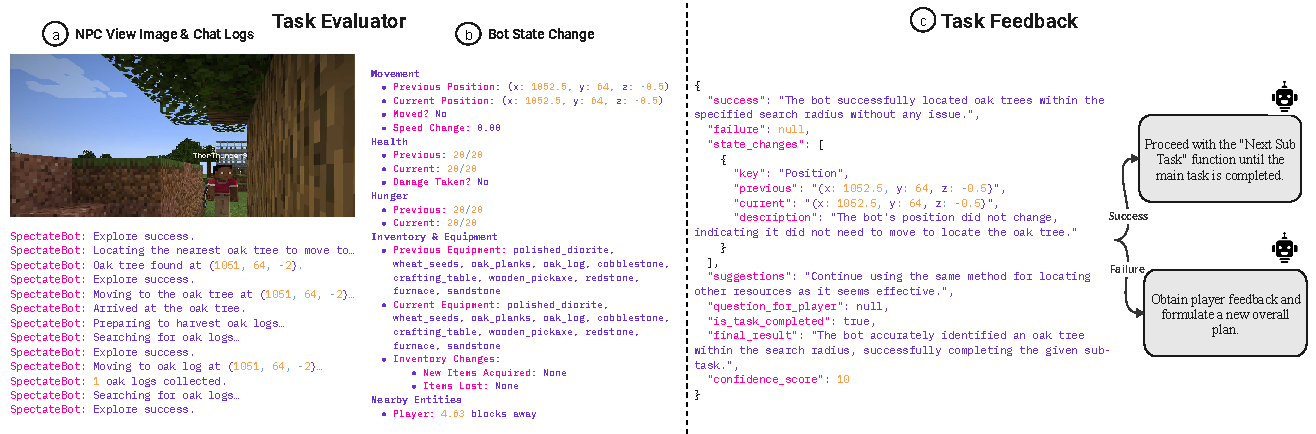
\includegraphics[width=1.0\textwidth]{Sections/Figures/task_feedback_fig.pdf}
  \captionof{figure}{Judging and repair. \panel{a} Evaluator consumes bounded evidence: a short window of recent chat and an NPC camera frame. \panel{b} State deltas between pre/post snapshots (position, inventory/equipment, nearby entities/blocks). \panel{c} Structured \texttt{TaskFeedback} with success/failure and rationale, state changes, suggestions, optional question for the player, and a confidence score.}
  \label{fig:taskfeedback}
\end{strip}

% \FloatBarrier
\FloatBarrier
% \clearpage
% \newpage